Murtolukujen lisäksi desimaaliluvut ovat tuttu tapa merkitä lukuja, jotka eivät ole kokonaislukuja. $123,456$ on esimerkki desimaaliluvusta. Pilkun jälkeen tulevat numerot tarkoittavat kymmenesosia, sadasosia ja niin edelleen.

\alakohdat{
	§ $123$ on sen \termi{kokonaisosa}{kokonaisosa}.
	§ Kokonaisluku erotetaan loppuosasta \termi{desimaalierotin}{desimaalierottimella}, joka on suomen kielessä pilkku (,)
	§ Osaa $456$ kutsutaan luvun \termi{desimaaliosa}{desimaaliosaksi}.
}

\laatikko[Desimaaliluku]{

Esimerkkinä annettu desimaaliluku tulkitaan seuraavasti:
\begin{equation*}
123,456 = 1 \cdot 10^2 + 2 \cdot 10^1 + 3 \cdot 10^0 + 4 \cdot 10^{-1} + 5 \cdot 10^{-2} + 6 \cdot 10^{-3}
\end{equation*}

\begin{equation*}
\huge \bf \underbrace{1}_{1\cdot10^2}\underbrace{2}_{2 \cdot 10^1}\underbrace{3}_{3 \cdot 10^0},\underbrace{4}_{4 \cdot 10^{-1}}\underbrace{5}_{5 \cdot 10^{-2}}\underbrace{6}_{6 \cdot 10^{-3}}
\end{equation*}

%FIXME kuvassa virhe, väärät kymmenpotenssien eksponentin desimaalipilkun vasemmalla puolella
%\begin{center}
% 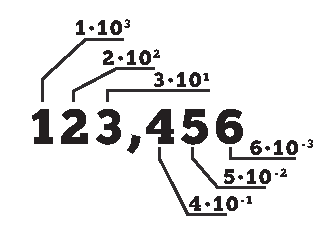
\includegraphics{pictures/Kuva5-1-desimaali-potenssit.pdf}
%\end{center}
}

Kymmenjärjestelmä saa nimensä siitä, että jokainen luvussa esiintyvä numeromerkki kertoo sen paikkaa vastaavien kymmenen potenssien määrän. %viittaus lukujärjestelmäliitteeseen

\subsection{Murtoluvun muuttaminen desimaaliluvuksi}

Murtoluku on tapa merkitä jakolaskua. Jakolaskun tuloksen esittämiseksi desimaalilukuna käytetään peruskoulun alaluokilla opetettavaa jakokulmaa. Jakokulman ajatus on yksinkertaisesti kokeilla, kuinka monta jakajaa, sen kymmenesosaa, sadasosaa ja niin edelleen jaettavaan mahtuu. Jakokulmat voi laskea käsin, laskin tekee saman nopeammin.

\begin{esimerkki}
Muutetaan $\frac{21}{4}$ desimaaliluvuksi laskemalla jakolasku $21:4$ jakokulmassa.
% v TÄMÄ v
% Voisiko laskuun selitää myös sanallisen selityksen siitä, mitä missäkin vaiheessa tapahtuu? Esim.
% Huomataan että luku 4 menee lukuun 21 viisi kertaa -> merkitään 5 jakokulman yläpuolelle ykkösten kohdalle.
% Tarkistetaan jakolasku kertolaskun avulla: $4 \cdot 5 = 20$. 
% Lasketaan jakojäännös erotuksena $21 - 20 = 1$.
% Luku 4 ei mene lukuun 1 yhtään kertaa, joten ``pudotetaan'' jaettavasta 0 desimaalierottimen oikealta puolelta (vastaukseen pitää muistaa merkitä desimaalierotin vastaavaan kohtaan kuin jaettavassa.) Luku 4 menee lukuun 10 kaksi kertaa -> merkitään 2 jakokulmaan kymmenesosien kohdalle.
% Tarkistetaan jakolasku kertolaskun avulla: $4 \cdot 2 = 8$, ja jakojäännökseksi jää $10 - 8 = 2$.
% \ldots
%
% Kun jakojäännökseksi jää luku nolla, jako on mennyt tasan ja vastaus on luettavissa jakokulman yläpuolelta.

%$\longdiv{21}{4}$

\[ 
\begin{array}{cccccc}
 & \underline{ \ \ } & \underline{5}, & \underline{2} & \underline{5} \\
 4 & \!\!|\,2 & 1, & 0 & 0 \\
 \underline{-} & \underline{2}& \underline{0} \\
 & & 1 &0 \\
 & \underline{-} &\underline{ \ \ }  & \underline{8} \\
 & & & 2 & 0 \\
 & & \underline{-} & \underline{2} & \underline{0} \\
 & &  & & 0
\end{array}
\]

Siis $21/4=5,25$.

%Jakolasku ei mene tasan, vaan jakojäännökseksi jää $1$. Siis $\frac{21}{4} = 5+\frac{1}{4} = 5,25$.

%$\longdiv{3}{11}$

Vastaavasti laskien saadaan $\frac{3}{11}=0,272727\ldots \ $ :
\[ 
\begin{array}{cccccc}
 & \underline{ 0}, & \underline{2} & \underline{7} & \underline{2} & 
 \underline{\ldots} \\
 11 & \!\!|\,3, & 0 & 0 & 0 & \ldots \\
 \underline{-} & \underline{2}& \underline{2} \\
 & & \boldsymbol{8} &0 \\
 & \underline{-} &\underline{ 7 }  & \underline{7} \\
 & & & \boldsymbol{3} & 0 \\
 & & \underline{-} & \underline{2} & \underline{2} \\
 & &  & & \boldsymbol{8} & 0 \\
 & & & & & \ddots
\end{array}
\]
Koska jakojäännökset $3$ ja $8$ toistuvat loputtomiin, tämä desimaaliluku ei ole päättyvä. Siinä on \termi{jakso}{jakso}: numerosarja $27$ toistuu. Jaksoa voidaan merkitä yläviivan avulla seuraavasti:
\[0,27272727\ldots = 0,\overline{27}\]
\end{esimerkki}

Tavan mukaan jakolaskun mennessä tasan desimaaliluvun tulevia nollia $\ldots000\ldots=\overline{0}$ ei merkitä, kuten ei nollia luvun edessäkään.

\begin{esimerkki}
	\alakohdat{
	§ $\frac{5}{4} = 1,250000\ldots = 1,25\overline{0}$ merkitään $1,25$
	§ $001,25$ merkitään $1,25$
	}
\end{esimerkki}

Huomaa, että matemaatikolle luvut $1,25$ ja $1,250$ tarkoittavat täsmälleen samaa asiaa. Sovelluksissa, joissa luvut eivät ole tarkkoja vain mittaustuloksia tai arvioita, esityksillä voi olla nyanssiero, joka kertoo mittauksen tarkkuudesta. Vastaustarkkuudesta ja pyöristämisestä kerrotaan lisää myöhemmin. %viittaus Yksiköt ja vastaustarkkuus -lukuun (jos se vielä sen niminen on)

Toistuva nollien jakso on vain yksi esimerkki rationaalilukujen desimaaliesityksen vääjäämättömästä jaksollisuudesta.

\laatikko[Rationaalilukujen desimaaliesitykset]{Kaikkien rationaalilukujen desimaaliesitykset ovat jaksollisia.}

Vähennyslaskuissa syntyvät jakojäännökset ovat nimittäin aina jakajaa pienempiä, ja siksi ne alkavat väistämättä toistaa itseään, ellei jako jossakin vaiheessa mene tasan. Koska eri vaihtoehtoja jakojäännöksiksi on yksi jakajaa vähemmän, jakson pituus on suurimmillaan yhden verran jakajaa pienempi. Esimerkiksi luvulla $\frac{1}{7}=0,\overline{142857}$ jakso on pisin mahdollinen, $7-1=6$ numeron mittainen.

\begin{esimerkki}
Esimerkkejä murtolukujen desimaaliesityksistä
\alakohdat{
	§ $ \frac{1}{10} = 0,1$
	§ $ \frac{1}{100} = 0,01$
	§ $ \frac{1}{2} = 0,5$
	§ $ \frac{1}{4} = 0,25$
	§ $ \frac{3}{4} = 0,75$
}
\end{esimerkki}


\subsection{Desimaaliluvun muuttaminen murtoluvuksi}

\termi{päättyvä desimaaliluku}{Päättyvät desimaaliluvut} voidaan muuttaa murtoluvuiksi muuttamalla kukin desimaali erikseen murtoluvuksi ja laskemalla syntyneet luvut yhteen.

\begin{esimerkki}
$21,37 = 21+ \frac{3}{10}+\frac{7}{100} =
\frac{2\,100}{100}+\frac{30}{100}+\frac{7}{100}
 = \frac{2\,100+30+7}{100} = \frac{2\,137}{100}.$
\end{esimerkki}

Tämä on turhan työlästä, ja paljon helpommalla päästäänkin laventamalla luku ''niin monella kympillä, kuin desimaalipilkun jälkeen on numeroita'' -- täsmällisemmin sanottuna laventamalla luvulla $10^n$, jossa $n$ on pilkun jälkeen tulevien numeroiden määrä.

\begin{esimerkki}
Luvussa $52,41$ kaksi desimaalia (pienimpinä sadasosat), joten lavennetaan siis sadalla. ($100=10^2$)
$52,41 = 52,41 \cdot  \frac{100}{100} = \frac{52,41 \cdot 100}{100} = \frac{5\,241}{100}$
\end{esimerkki}

\begin{esimerkki}
$0,007 = 0,007 \cdot 1 = 0,007 \cdot \frac{10^3}{10^3} = \frac{0,007 \cdot 1\,000}{1\,000} = \frac{7}{1\,000}$
\end{esimerkki}

(Muista, että erilaisia murtolukuesityksiä on kuitenkin olemassa samalle luvulle ääretön määrä. Saattaa olla, että menetelmällä saatu murtoluku on vielä supistettavissa.)
%Menetelmän toimivuus kaikkien desimaalilukujen tapauksessa voidaan todistaa %tarkastelemalla desimaaliluvun määritelmää, mutta jätetään tässä tekemättä.

Minkä tahansa \termi{jaksollinen desimaaliluku}{jaksollisen desimaaliluvun} voi muuttaa murtoluvuksi seuraavalla tempulla: Muutetaan esimerkiksi $0,575757\ldots$ murtoluvuksi. Jos merkitään
\[
\begin{array}{rcll}
x &=& \ \, 0,575757 \ldots\ , &\textrm{saadaan sadalla kertomalla} \\
100x &=& 57,575757 \ldots \ , &\textrm{joiden erotuksena} \\
100x - x &=& 57,57 \ldots - 0,57 \ldots \ , & \textrm{eli} \\
99x &=& 57, & \textrm{josta saadaan} \\
x &=& \frac{57}{99} = \frac{19}{33}.
\end{array}
\]
Siis $0,575757\ldots = \frac{19}{33}$. Menetelmä toimii kaikille jaksollisille desimaaliluvuille: kerrotaan vain sopivalla luvun $10$ potenssilla, jotta jakso katoaa vähennyslaskussa.

\luettelolaatikko{Nämä kannattaa muistaa}{
§ $\frac{1}{3} = 0,3333\ldots$
§ $\frac{2}{3} = 0,6666\ldots$
}
